\PilotPage{20}

\begin{align}
    u_0=u(0)&=A\cos\omega_n t+B\sin\omega_n t\big|_{t=0}=A, \notag\\
    \dot{u}_0=\dot{u}(0)&=-\omega_n A\sin\omega_n t+\omega_n B\cos\omega_n t\big|_{t=0}=\omega_n B. \tag{23}
\end{align}
Solving Eq.~(23) for $A$ and $B$ yields
\begin{align}
    A&=u_0, \notag\\
    B&=\frac{\dot{u}_0}{\omega_n}. \tag{24}
\end{align}
Substitution of Eq.~(24) into Eq.~(18) gives the general solution of undamped free vibrations with initial displacement, $u_0$, and initial velocity, $\dot{u}_0$, in the form
\begin{equation}
    u(t)=u_0\cos\omega_n t+\frac{\dot{u}_0}{\omega_n}\sin\omega_n t. \tag{25}
\end{equation}

\subsubsection{Vertical spring--mass analysis}

So far, we have assumed the mass--spring vibrating system is horizontal. However, many spring--mass vibrating systems are vertical. In this section, we show that a vertical spring--mass obeys the same differential equation as a horizontal one, which means that the analysis outlined so far applies equally to both situations.

\setcounter{figure}{1}
\begin{figure}[!ht]
  \centering
  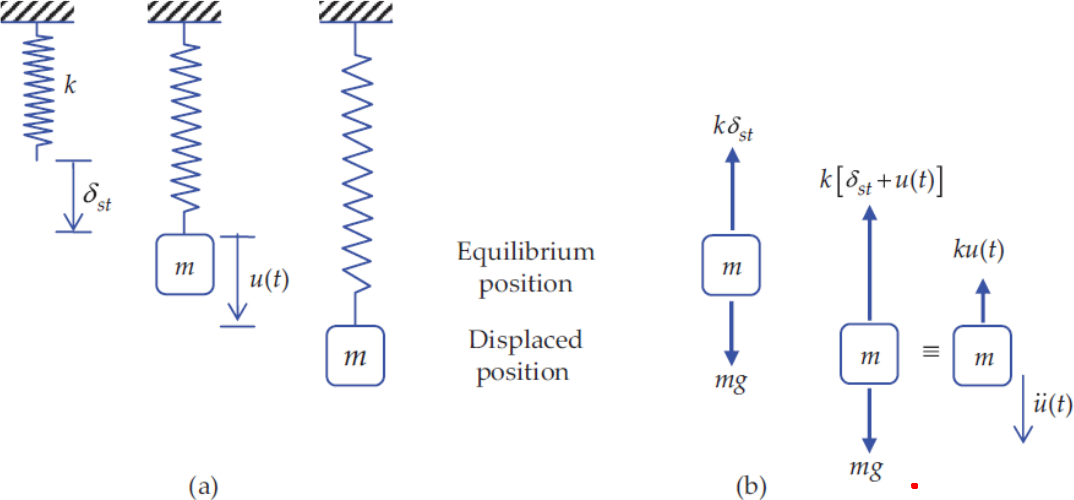
\includegraphics[
    max width=0.93\linewidth,
    max height=1.72in,
  ]{figures/p020-vertical-spring-mass.png}
  \caption{Free vibration of a vertical spring-mass system: (a) physical mechanism; (b) free-body diagram}
\end{figure}
